\chapter{The Mole and Molar Mass}\label{ch:g10:the-mole}

At the end of the day, a bank does not count its coins one by one: it
weighs them. If one coin has a mass of \qty{7.5}{g}, a bag of coins with
a mass of \qty{7.5}{kg} holds a thousand coins, and the scale has done
the counting. Chemists face the same problem with \omterm{def:g7:atoms-and-molecules:atom}{atoms}, only far worse:
a spoonful of water holds more \omterm{def:g7:atoms-and-molecules:molecule}{molecules} than there are grains of sand
on all the beaches of a coast. They solve it the same way, by weighing,
and the bag they use holds
\num{602214076000000000000000} entities. This chapter defines that bag,
the \omterm{def:g10:the-mole:amount}{mole}, and shows how to go from a mass on a balance to a number of
\omterm{def:g7:atoms-and-molecules:atom}{atoms} or \omterm{def:g7:atoms-and-molecules:molecule}{molecules}.

\begin{recall}
The mass of an \omterm{def:g7:atoms-and-molecules:atom}{atom} is concentrated in its \omterm{def:g9:inside-the-atom:nucleus}{nucleus}; a \omterm{def:g9:inside-the-atom:proton}{proton} and a
\omterm{def:g9:inside-the-atom:proton}{neutron} each have a mass of about \qty{1.67e-27}{kg}, so an \omterm{def:g7:atoms-and-molecules:atom}{atom} of \omterm{def:g9:inside-the-atom:atomic-number}{mass
number} $A$ has a mass of about $A \times \qty{1.67e-27}{kg}$. Large and
small numbers are written in scientific notation
(\cref{ch:g9:inside-the-atom}). A \omterm{def:g7:atoms-and-molecules:formula}{chemical formula} gives the number of
\omterm{def:g7:atoms-and-molecules:atom}{atoms} of each element in a \omterm{def:g7:atoms-and-molecules:molecule}{molecule} (\cref{ch:g7:atoms-and-molecules}).
\end{recall}

\begin{omfigure}
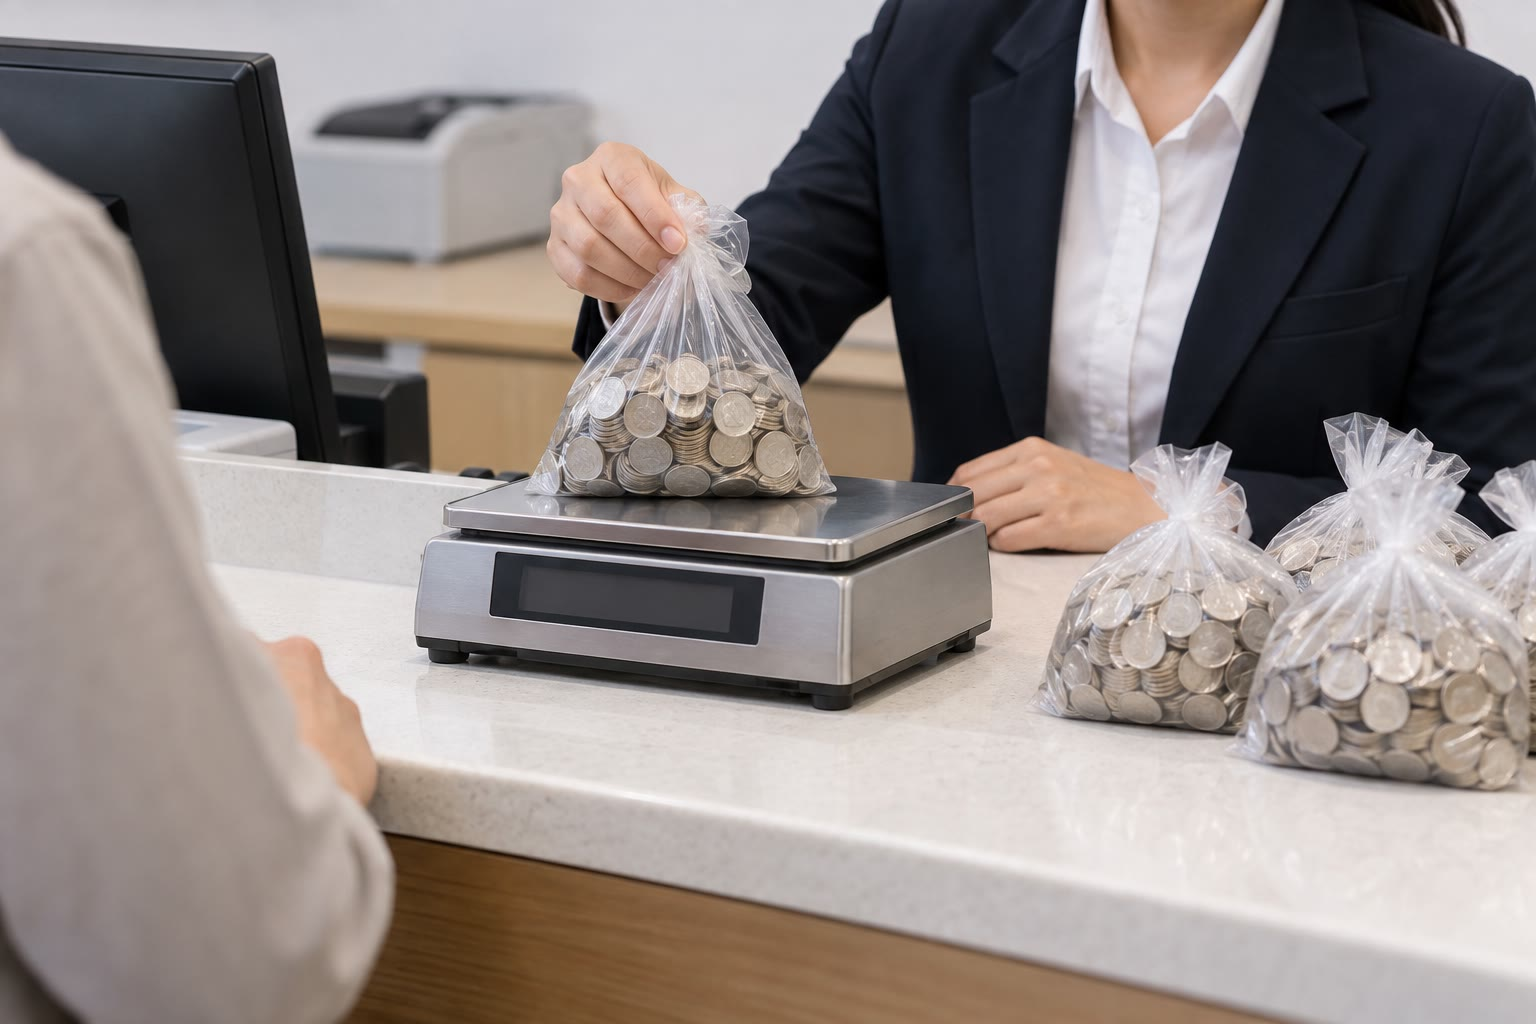
\includegraphics[width=0.55\linewidth]{images/book1/ai/g10-bank-coins.jpg}

{\small A bank counts coins by weighing them. Chemists count \omterm{def:g7:atoms-and-molecules:atom}{atoms} the
same way.}
\end{omfigure}

\section{Counting by weighing}

\begin{example}[A bag of coins]\label{ex:g10:the-mole:coins}
A coin has a mass of \qty{7.5}{g}. A bag of these coins has a mass of
\qty{1.80}{kg}, that is \qty{1800}{g}, the mass of the bag itself left
aside. It holds
\[
  \frac{\qty{1800}{g}}{\qty{7.5}{g}} = 240 \text{ coins.}
\]
To count, the bank divides the total mass by the mass of one coin.
\end{example}

\begin{example}[A spoonful of water]\label{ex:g10:the-mole:spoon}
A water \omterm{def:g7:atoms-and-molecules:molecule}{molecule}, \ce{H2O}, has $2 + 16 = 18$ \omterm{def:g9:inside-the-atom:proton}{nucleons} (the oxygen-16
and hydrogen-1 \omterm{def:g7:atoms-and-molecules:atom}{atoms} make up nearly all natural water), so its mass is
about $18 \times \qty{1.67e-27}{kg} = \qty{3.0e-26}{kg}$, or
\qty{3.0e-23}{g}. A spoonful of \qty{5.0}{g} of water therefore holds
\[
  \frac{\qty{5.0}{g}}{\qty{3.0e-23}{g}} \approx \num{1.7e23}
  \text{ molecules.}
\]
The division works as for the coins, but the answer is a number no one
can picture. Chemists need a package of \omterm{def:g7:atoms-and-molecules:atom}{atoms} adapted to the samples of
the laboratory.
\end{example}

\begin{definition}[Amount of substance and mole]\label{def:g10:the-mole:amount}
% ledger: const:NA
The \emph{amount of substance}\index{amount of substance} $n$ of a sample
counts the entities it contains (\omterm{def:g7:atoms-and-molecules:atom}{atoms}, \omterm{def:g7:atoms-and-molecules:molecule}{molecules} or \omterm{def:g9:ions:ion}{ions}, stated each
time). Its unit is the \emph{mole}\index{mole}, symbol \si{mol}: one mole
contains exactly \num{6.02214076e23} entities.
\end{definition}

\begin{remark}[A dozen, a ream, a mole]\label{rem:g10:the-mole:dozen}
The \omterm{def:g10:the-mole:amount}{mole} is a counting unit, like a dozen eggs (12) or a ream of paper
(500 sheets), only very much larger. ``Two \omterm{def:g10:the-mole:amount}{moles} of water \omterm{def:g7:atoms-and-molecules:molecule}{molecules}''
means $2 \times \num{6.02214076e23} = \num{1.20e24}$ \omterm{def:g7:atoms-and-molecules:molecule}{molecules}, just as
``two dozen eggs'' means 24 eggs. Always say which entities are counted:
one \omterm{def:g10:the-mole:amount}{mole} of oxygen \emph{\omterm{def:g7:atoms-and-molecules:molecule}{molecules}} \ce{O2} holds two \omterm{def:g10:the-mole:amount}{moles} of oxygen
\emph{\omterm{def:g7:atoms-and-molecules:atom}{atoms}}.
\end{remark}

\begin{history}[Avogadro's hypothesis, 1811]
In 1811 the physicist Amedeo Avogadro proposed that equal
volumes of different gases, at the same temperature and pressure,
contain the same number of particles. He also understood that a gas such
as oxygen is made of \omterm{def:g7:atoms-and-molecules:molecule}{molecules} of two \omterm{def:g7:atoms-and-molecules:atom}{atoms}. His idea was neglected for
nearly fifty years, until Stanislao Cannizzaro used it in 1860 to obtain
a coherent set of atomic weights. The constant that counts the entities
of a \omterm{def:g10:the-mole:amount}{mole} was later named after Avogadro; he never knew its value.
\end{history}

\begin{omfigure}
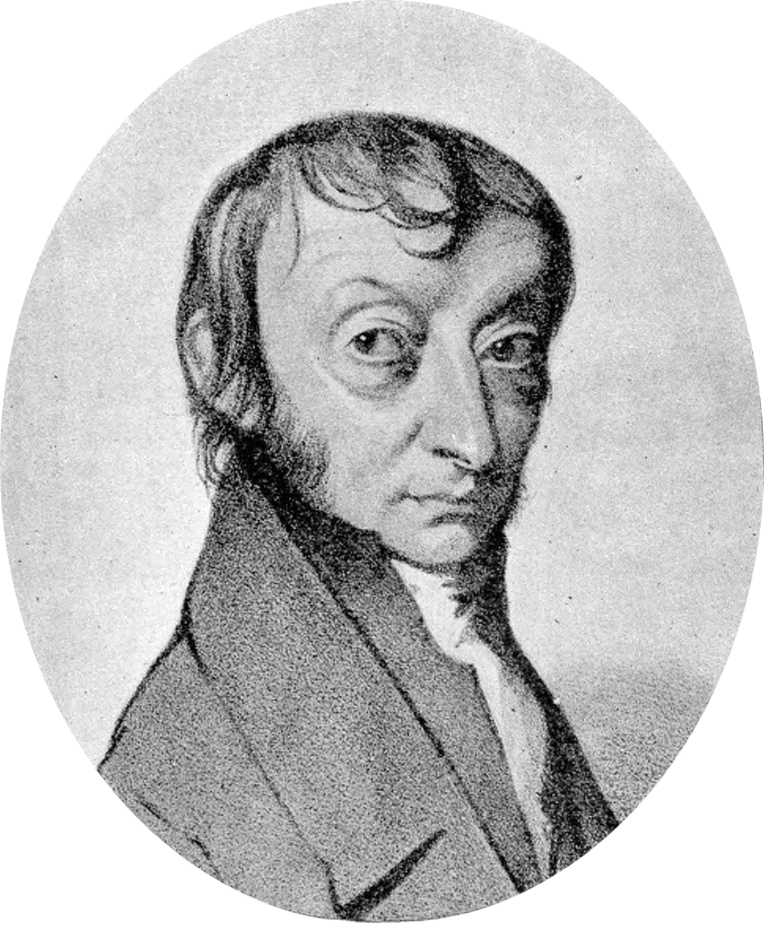
\includegraphics[width=0.26\linewidth]{images/book1/avogadro.jpg}

{\small Amedeo Avogadro (1776--1856).}
\end{omfigure}

\section{The Avogadro constant}

\begin{definition}[Avogadro constant]\label{def:g10:the-mole:avogadro}
% ledger: const:NA
The \emph{Avogadro constant}\index{Avogadro constant} $N_A$ is the
number of entities per \omterm{def:g10:the-mole:amount}{mole}:
\[
  N_A = \qty{6.02214076e23}{mol^{-1}} .
\]
Its value is exact, fixed by definition. In calculations it is rounded
to \qty{6.02e23}{mol^{-1}}.
\end{definition}

\begin{proposition}[Number of entities and amount]\label{prop:g10:the-mole:number}
A sample holding $N$ entities contains the amount
\[
  n = \frac{N}{N_A}, \qquad\text{that is}\qquad N = n \times N_A .
\]
\end{proposition}

\begin{proof}
Each \omterm{def:g10:the-mole:amount}{mole} contains $N_A$ entities, so $n$ \omterm{def:g10:the-mole:amount}{moles} contain $n \times N_A$
entities; dividing by $N_A$ gives $n$.
\end{proof}

\begin{example}[Molecules and moles]\label{ex:g10:the-mole:convert}
A sample contains \num{1.5e24} \omterm{def:g7:atoms-and-molecules:molecule}{molecules} of carbon dioxide. Its amount
of carbon dioxide is
$n = \num{1.5e24} / \qty{6.02e23}{mol^{-1}} = \qty{2.5}{mol}$.
Conversely, \qty{0.20}{mol} of iron holds
$N = \qty{0.20}{mol} \times \qty{6.02e23}{mol^{-1}} = \num{1.2e23}$
\omterm{def:g7:atoms-and-molecules:atom}{atoms} of iron.
\end{example}

\begin{remark}[Where the number comes from]\label{rem:g10:the-mole:origin}
For more than fifty years the \omterm{def:g10:the-mole:amount}{mole} was defined as the number of \omterm{def:g7:atoms-and-molecules:atom}{atoms} in
exactly \qty{12}{g} of carbon-12, and $N_A$ had to be measured. Since
2019 the number itself has been fixed, which makes the \omterm{def:g10:the-mole:amount}{mole} a pure count.
The old and new definitions agree to better than one part in a
hundred million, so twelve grams of carbon-12 still contain one \omterm{def:g10:the-mole:amount}{mole} of
\omterm{def:g7:atoms-and-molecules:atom}{atoms}, as the next section checks.
\end{remark}

\section{Molar mass}

\begin{definition}[Molar mass]\label{def:g10:the-mole:molar-mass}
The \emph{molar mass}\index{molar mass} $M$ of a \omterm{def:g6:pure-substances-and-mixtures:species}{chemical species} is the
mass of one \omterm{def:g10:the-mole:amount}{mole} of its entities, in grams per \omterm{def:g10:the-mole:amount}{mole} (\si{g/mol}). The
molar mass of an element, taken over its natural \omterm{def:g6:pure-substances-and-mixtures:mixture}{mixture} of \omterm{def:g9:inside-the-atom:isotope}{isotopes}, is
its \emph{atomic molar mass}\index{atomic molar mass}; it is printed in
the \omterm{def:g9:periodic-table-first-look:periodic-table}{periodic table}.
\end{definition}

\begin{example}[One mole of carbon atoms]\label{ex:g10:the-mole:carbon}
% ledger: const:NA, const:u
An \omterm{def:g7:atoms-and-molecules:atom}{atom} of carbon-12 has a mass of about
$12 \times \qty{1.67e-27}{kg} = \qty{2.00e-26}{kg}$. One \omterm{def:g10:the-mole:amount}{mole} of them
has a mass of
\[
  \qty{2.00e-26}{kg} \times \num{6.02e23} = \qty{1.20e-2}{kg}
  = \qty{12.0}{g}.
\]
The \omterm{def:g10:the-mole:amount}{mole} has been chosen so that the \omterm{def:g10:the-mole:molar-mass}{molar mass} of an \omterm{def:g7:atoms-and-molecules:atom}{atom}, in grams per
\omterm{def:g10:the-mole:amount}{mole}, is close to its \omterm{def:g9:inside-the-atom:atomic-number}{mass number}: about \qty{1}{g/mol} for hydrogen,
\qty{12}{g/mol} for carbon, \qty{16}{g/mol} for oxygen.
\end{example}

\begin{omfigure}
% ledger: aw:H, aw:C, aw:N, aw:O, aw:Na, aw:Mg, aw:Al, aw:Si, aw:S, aw:Cl, aw:K, aw:Ca, aw:Fe, aw:Cu, aw:Zn, aw:Au (rounded to 0.1)
\begin{tabular}{lcr@{\qquad}lcr}
\hline
element & symbol & $M$ (\si{g/mol}) & element & symbol & $M$ (\si{g/mol}) \\
\hline
hydrogen  & \ce{H}  & 1.0  & silicon   & \ce{Si} & 28.1 \\
carbon    & \ce{C}  & 12.0 & sulfur    & \ce{S}  & 32.1 \\
nitrogen  & \ce{N}  & 14.0 & chlorine  & \ce{Cl} & 35.5 \\
oxygen    & \ce{O}  & 16.0 & potassium & \ce{K}  & 39.1 \\
sodium    & \ce{Na} & 23.0 & calcium   & \ce{Ca} & 40.1 \\
magnesium & \ce{Mg} & 24.3 & iron      & \ce{Fe} & 55.8 \\
aluminium & \ce{Al} & 27.0 & copper    & \ce{Cu} & 63.5 \\
          &         &      & gold      & \ce{Au} & 197.0 \\
\hline
\end{tabular}\par\medskip

{\small Atomic molar masses of common elements, rounded to
\qty{0.1}{g/mol}. These are the values used in this book.}
\end{omfigure}

\begin{remark}[Why chlorine is 35.5]\label{rem:g10:the-mole:chlorine}
% ledger: iso:Cl35, iso:Cl37
Natural chlorine is a \omterm{def:g6:pure-substances-and-mixtures:mixture}{mixture} of two \omterm{def:g9:inside-the-atom:isotope}{isotopes}: about three quarters of
its \omterm{def:g7:atoms-and-molecules:atom}{atoms} are chlorine-35, one quarter chlorine-37
(\cref{ch:g9:inside-the-atom}). Its \omterm{def:g10:the-mole:molar-mass}{atomic molar mass} is the average,
weighted by these shares, which lies between 35 and 37: \qty{35.5}{g/mol}.
That is why some atomic molar masses are far from whole numbers.
\end{remark}

\begin{proposition}[Molar mass of a molecule]\label{prop:g10:the-mole:sum}
The \omterm{def:g10:the-mole:molar-mass}{molar mass} of a \omterm{def:g7:atoms-and-molecules:molecule}{molecule} is the sum of the atomic molar masses of all
its \omterm{def:g7:atoms-and-molecules:atom}{atoms}, each counted as many times as it appears in the formula. The
same rule gives the \omterm{def:g10:the-mole:molar-mass}{molar mass} of an ionic solid from its formula unit.
\end{proposition}

\begin{proof}
One \omterm{def:g10:the-mole:amount}{mole} of \omterm{def:g7:atoms-and-molecules:molecule}{molecules} \ce{A_xB_y} contains $x$ \omterm{def:g10:the-mole:amount}{moles} of \omterm{def:g7:atoms-and-molecules:atom}{atoms} \ce{A} and
$y$ \omterm{def:g10:the-mole:amount}{moles} of \omterm{def:g7:atoms-and-molecules:atom}{atoms} \ce{B}, and nothing else; its mass is the sum of their
masses, $x\,M(\ce{A}) + y\,M(\ce{B})$.
\end{proof}

\begin{example}[Three molar masses]\label{ex:g10:the-mole:three}
% ledger: aw:H, aw:C, aw:O, aw:Na, aw:Cl
\begin{align*}
  M(\ce{H2O}) &= 2 \times 1.0 + 16.0 = \qty{18.0}{g/mol},\\
  M(\ce{NaCl}) &= 23.0 + 35.5 = \qty{58.5}{g/mol},\\
  M(\ce{C12H22O11}) &= 12 \times 12.0 + 22 \times 1.0 + 11 \times 16.0
     = \qty{342.0}{g/mol}.
\end{align*}
The last one is sucrose, table sugar.
\end{example}

\section{From mass to amount and back}

\begin{proposition}[Mass and amount]\label{prop:g10:the-mole:mass}
A sample of mass $m$ of a species of \omterm{def:g10:the-mole:molar-mass}{molar mass} $M$ contains the amount
\[
  n = \frac{m}{M}, \qquad\text{that is}\qquad m = n \times M .
\]
With $m$ in grams and $M$ in grams per \omterm{def:g10:the-mole:amount}{mole}, $n$ is in \omterm{def:g10:the-mole:amount}{moles}.
\end{proposition}

\begin{proof}
Each \omterm{def:g10:the-mole:amount}{mole} has a mass $M$, so $n$ \omterm{def:g10:the-mole:amount}{moles} have a mass $n \times M$; this is
the coin count of the bank, with the \omterm{def:g10:the-mole:amount}{mole} as the coin.
\end{proof}

\begin{method}[From a mass to a number of entities]\label{met:g10:the-mole:mass-to-number}
\begin{enumerate}
  \item Write the formula of the species and compute its \omterm{def:g10:the-mole:molar-mass}{molar mass} $M$
        from the table.
  \item Convert the mass to grams if needed, then $n = m / M$.
  \item If the number of entities is wanted, $N = n \times N_A$.
  \item Check the order of magnitude: a few grams of a small \omterm{def:g7:atoms-and-molecules:molecule}{molecule} is
        of the order of a tenth of a \omterm{def:g10:the-mole:amount}{mole}, some $10^{22}$ to $10^{23}$
        entities.
\end{enumerate}
\end{method}

\begin{omfigure}
\begin{tikzpicture}[font=\small, box/.style={draw=omDef, very thick,
    fill=omDef!8, rounded corners=3pt, minimum width=2.9cm,
    minimum height=1.1cm, align=center}]
  \node[box] (m) at (0,0) {mass $m$\\[1pt] (\si{g})};
  \node[box] (n) at (5,0) {amount $n$\\[1pt] (\si{mol})};
  \node[box] (N) at (10,0) {number $N$\\[1pt] of entities};
  \draw[-{Stealth[length=7pt]}, thick, omProp] ([yshift=4pt]m.east)
    -- node[above] {$\div M$} ([yshift=4pt]n.west);
  \draw[-{Stealth[length=7pt]}, thick, omProp] ([yshift=-4pt]n.west)
    -- node[below] {$\times M$} ([yshift=-4pt]m.east);
  \draw[-{Stealth[length=7pt]}, thick, omProp] ([yshift=4pt]n.east)
    -- node[above] {$\times N_A$} ([yshift=4pt]N.west);
  \draw[-{Stealth[length=7pt]}, thick, omProp] ([yshift=-4pt]N.west)
    -- node[below] {$\div N_A$} ([yshift=-4pt]n.east);
\end{tikzpicture}

{\small The amount $n$ sits in the middle: the balance gives $m$, the
\omterm{def:g10:the-mole:molar-mass}{molar mass} leads to $n$, and the \omterm{def:g10:the-mole:avogadro}{Avogadro constant} leads on to the
number of entities.}
\end{omfigure}


\begin{example}[Nine grams of water]\label{ex:g10:the-mole:nine}
% ledger: aw:H, aw:O, const:NA
How many \omterm{def:g7:atoms-and-molecules:molecule}{molecules} are there in \qty{9.0}{g} of water? $M(\ce{H2O}) =
\qty{18.0}{g/mol}$, so
\[
  n = \frac{\qty{9.0}{g}}{\qty{18.0}{g/mol}} = \qty{0.50}{mol},
  \qquad
  N = \qty{0.50}{mol} \times \qty{6.02e23}{mol^{-1}}
    = \num{3.0e23} \text{ molecules.}
\]
\end{example}

\begin{example}[A mole on the bench]\label{ex:g10:the-mole:bench}
% ledger: rho:water, rho:NaCl, rho:sucrose, rho:Fe, aw:H, aw:O, aw:Na, aw:Cl, aw:C, aw:Fe
One \omterm{def:g10:the-mole:amount}{mole} of water is \qty{18.0}{g}, about a tablespoon. One \omterm{def:g10:the-mole:amount}{mole} of salt,
\qty{58.5}{g}, is a small heap; one \omterm{def:g10:the-mole:amount}{mole} of sugar, \qty{342.0}{g}, fills
a mug; one \omterm{def:g10:the-mole:amount}{mole} of iron, \qty{55.8}{g}, is a cube a little under
\qty{2}{cm} across. All four hold the same number of entities: the
\omterm{def:g7:atoms-and-molecules:molecule}{molecules} of sugar are simply much heavier than those of water, and the
\omterm{def:g7:atoms-and-molecules:atom}{atoms} of iron are packed much more tightly.
\end{example}

\begin{omfigure}
\begin{tikzpicture}[font=\small, x=0.62cm, y=0.62cm]
  % cubes of true volume, drawn to one common scale: side = cube root of V
  % water 18.09 cm3 -> 2.625 cm; NaCl 26.96 cm3 -> 2.999 cm;
  % sucrose 216.4 cm3 -> 6.004 cm; Fe 7.09 cm3 -> 1.921 cm
  \newcommand{\cube}[4]{% x, side, fill, label
    \pgfmathsetmacro\d{0.35*#2}
    \fill[#3!35, draw=#3!80!black] (#1,0) rectangle ++(#2,#2);
    \fill[#3!20, draw=#3!80!black] (#1,#2) -- ++(\d,\d) -- ++(#2,0)
      -- ++(-\d,-\d) -- cycle;
    \fill[#3!50, draw=#3!80!black] (#1+#2,0) -- ++(\d,\d) -- ++(0,#2)
      -- ++(-\d,-\d) -- cycle;
    \node[below, align=center] at (#1+#2/2,-0.1) {#4};}
  \cube{0}{2.625}{cyan}{water\\ \qty{18.0}{g}\\ \qty{18}{cm^3}}
  \cube{4.3}{2.999}{gray}{salt\\ \qty{58.5}{g}\\ \qty{27}{cm^3}}
  \cube{9}{6.004}{orange}{sugar\\ \qty{342.0}{g}\\ \qty{216}{cm^3}}
  \cube{18}{1.921}{brown}{iron\\ \qty{55.8}{g}\\ \qty{7}{cm^3}}
\end{tikzpicture}

{\small One \omterm{def:g10:the-mole:amount}{mole} each of water, salt (sodium chloride), sugar (sucrose)
and iron, drawn as cubes of their true volumes, all at the same scale.
Each holds \num{6.02e23} entities.}
\end{omfigure}

\section{Gases: the molar volume}

\begin{definition}[Molar volume]\label{def:g10:the-mole:molar-volume}
The \emph{molar volume}\index{molar volume} $V_m$ of a gas is the volume
occupied by one \omterm{def:g10:the-mole:amount}{mole} of that gas, at a given temperature and pressure.
It is expressed in litres per \omterm{def:g10:the-mole:amount}{mole} (\si{L/mol}).
\end{definition}

\begin{proposition}[All gases have the same molar volume]\label{prop:g10:the-mole:avogadro-law}
% ledger: const:R, const:atm, const:Vm1 (24.1 = R x 293.15 K / 101325 Pa, computed)
At a given temperature and pressure, one \omterm{def:g10:the-mole:amount}{mole} of any gas occupies very
nearly the same volume, whatever the gas. At \qty{20}{\celsius} and
normal atmospheric pressure,
\[
  V_m = \qty{24.1}{L/mol};
\]
at \qty{0}{\celsius} and the same pressure, $V_m = \qty{22.4}{L/mol}$. The
amount of a gas of volume $V$ is then $n = V / V_m$.
\end{proposition}

\begin{proof}
Admitted here: this is Avogadro's hypothesis of 1811, now a law of
physics, and the value of $V_m$ follows from the gas laws studied in the
physics book.
\end{proof}

\begin{omfigure}
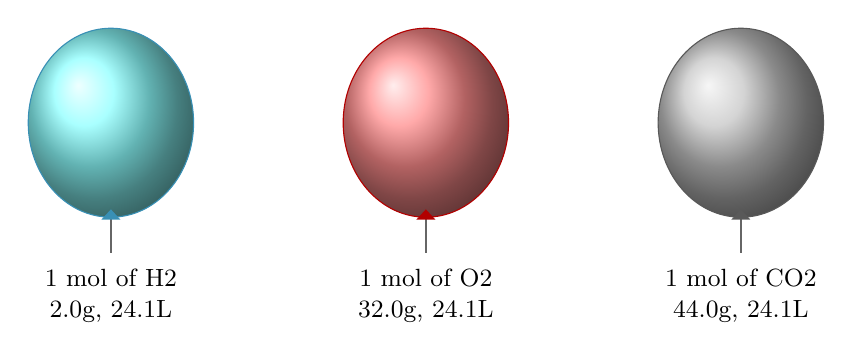
\begin{tikzpicture}[font=\small]
  \foreach \x/\g/\m/\c in {0/{\ce{H2}}/2.0/cyan, 4/{\ce{O2}}/32.0/red,
                           8/{\ce{CO2}}/44.0/gray} {
    \draw[thick, black!60] (\x,-0.25) -- (\x,-1.1);
    \shade[ball color=\c!45, draw=\c!70!black] (\x,0.55) ellipse (1.05 and 1.2);
    \fill[\c!70!black] (\x-0.12,-0.68) -- (\x+0.12,-0.68) -- (\x,-0.55) -- cycle;
    \node[align=center] at (\x,-1.65) {1 mol of \g\\ \qty{\m}{g},
      \qty{24.1}{L}};
  }
\end{tikzpicture}

{\small Three balloons at \qty{20}{\celsius}, each holding one \omterm{def:g10:the-mole:amount}{mole} of a
different gas. The volumes are the same; the masses are not.}
\end{omfigure}


\begin{example}[A balloon of carbon dioxide]\label{ex:g10:the-mole:balloon}
% ledger: aw:C, aw:O
A balloon holds \qty{2.4}{L} of carbon dioxide at \qty{20}{\celsius}.
Its amount is $n = \qty{2.4}{L} / \qty{24.1}{L/mol} = \qty{0.10}{mol}$,
and its mass $m = \qty{0.10}{mol} \times \qty{44.0}{g/mol} =
\qty{4.4}{g}$. The same balloon filled with hydrogen would hold the same
\qty{0.10}{mol}, but only \qty{0.20}{g} of gas.
\end{example}

\begin{remark}[Heavy and light gases]\label{rem:g10:the-mole:heavy}
Since a litre of any gas holds the same amount, the mass of a litre of
gas is proportional to its \omterm{def:g10:the-mole:molar-mass}{molar mass}. \omterm{def:g4:air-a-mixture-of-gases:air}{Air}, a \omterm{def:g6:pure-substances-and-mixtures:mixture}{mixture} of about four
fifths nitrogen (\qty{28.0}{g/mol}) and one fifth oxygen
(\qty{32.0}{g/mol}), behaves like a gas of \omterm{def:g10:the-mole:molar-mass}{molar mass} about
\qty{29}{g/mol}. A gas of larger \omterm{def:g10:the-mole:molar-mass}{molar mass}, such as carbon dioxide
(\qty{44.0}{g/mol}), is denser than \omterm{def:g4:air-a-mixture-of-gases:air}{air} and gathers at the bottom of a
closed cellar; a gas of smaller \omterm{def:g10:the-mole:molar-mass}{molar mass}, such as helium
(\qty{4.0}{g/mol}), rises.
\end{remark}

\section{Exercises}

\begin{exercise}[$\star$]\label{exo:g10:the-mole:1}
Compute the molar masses of dioxygen \ce{O2}, dinitrogen \ce{N2},
methane \ce{CH4}, ammonia \ce{NH3} and carbon dioxide \ce{CO2}.
\end{exercise}

\begin{exercise}[$\star$]\label{exo:g10:the-mole:2}
What \omterm{def:g10:the-mole:amount}{amount of substance} is contained in \qty{36.0}{g} of water? In
\qty{4.0}{g} of methane?
\end{exercise}

\begin{exercise}[$\star$]\label{exo:g10:the-mole:3}
What is the mass of \qty{0.25}{mol} of sodium chloride \ce{NaCl}? Of
\qty{2.0}{mol} of carbon dioxide?
\end{exercise}

\begin{exercise}[$\star$]\label{exo:g10:the-mole:4}
How many \omterm{def:g7:atoms-and-molecules:molecule}{molecules} are there in \qty{0.50}{mol} of dioxygen? What amount
of iron contains \num{3.0e24} \omterm{def:g7:atoms-and-molecules:atom}{atoms} of iron?
\end{exercise}

\begin{exercise}[$\star$]\label{exo:g10:the-mole:5}
At \qty{20}{\celsius} and normal atmospheric pressure, what volume does
\qty{0.50}{mol} of dinitrogen occupy? What amount of dioxygen is there in
\qty{12}{L} of that gas?
\end{exercise}

\begin{exercise}[$\star\star$]\label{exo:g10:the-mole:6}
A drop of water has a volume of \qty{0.050}{mL}, and \qty{1}{mL} of water
has a mass of \qty{1.0}{g}. How many water \omterm{def:g7:atoms-and-molecules:molecule}{molecules} does the drop
contain?
\end{exercise}

\begin{exercise}[$\star\star$]\label{exo:g10:the-mole:7}
Which contains more \omterm{def:g7:atoms-and-molecules:atom}{atoms}, \qty{10}{g} of aluminium or \qty{10}{g} of
iron? Explain without computing first, then check by computing.
\end{exercise}

\begin{exercise}[$\star\star$]\label{exo:g10:the-mole:8}
At \qty{20}{\celsius}, compute the mass of one litre of carbon dioxide
and of one litre of dinitrogen. Why does carbon dioxide collect at the
bottom of a closed cellar where grape juice is fermenting?
\end{exercise}

\begin{exercise}[$\star\star$]\label{exo:g10:the-mole:9}
Using the figure of the three boxes $m$, $n$, $N$, give the mass of
\num{1.0e22} \omterm{def:g7:atoms-and-molecules:molecule}{molecules} of glucose \ce{C6H12O6}. Write down the two
arrows followed.
\end{exercise}

\begin{exercise}[$\star\star$]\label{exo:g10:the-mole:10}
A lump of sugar (sucrose, \ce{C12H22O11}) has a mass of \qty{5.0}{g}.
Compute the amount of sucrose it contains, then the number of sucrose
\omterm{def:g7:atoms-and-molecules:molecule}{molecules}, then the number of carbon \omterm{def:g7:atoms-and-molecules:atom}{atoms}.
\end{exercise}

\begin{exercise}[$\star\star$]\label{exo:g10:the-mole:11}
Which contains the larger amount of \omterm{def:g7:atoms-and-molecules:molecule}{molecules}: \qty{1.0}{kg} of water
\ce{H2O} or \qty{1.0}{kg} of ethanol \ce{C2H6O}? By what factor?
\end{exercise}

\begin{exercise}[$\star\star\star$]\label{exo:g10:the-mole:12}
A gold ring has a mass of \qty{5.0}{g}; three quarters of its mass is
gold, the rest copper. How many \omterm{def:g7:atoms-and-molecules:atom}{atoms} of gold does it contain? How many
\omterm{def:g7:atoms-and-molecules:atom}{atoms} of copper? Which \omterm{def:g9:periodic-table-first-look:metal}{metal} has more \omterm{def:g7:atoms-and-molecules:atom}{atoms} in the ring?
\end{exercise}

\begin{exercise}[$\star\star\star$]\label{exo:g10:the-mole:13}
A classroom measures \qty{8.0}{m} by \qty{6.0}{m} by \qty{3.0}{m}, and
the \omterm{def:g4:air-a-mixture-of-gases:air}{air} in it is at \qty{20}{\celsius}.
\begin{enumerate}
  \item What amount of gas does it contain ($\qty{1}{m^3} =
        \qty{1000}{L}$)? How many \omterm{def:g7:atoms-and-molecules:molecule}{molecules}?
  \item Taking \omterm{def:g4:air-a-mixture-of-gases:air}{air} as 78 \omterm{def:g7:atoms-and-molecules:molecule}{molecules} of dinitrogen, 21 of dioxygen and 1 of
        argon (\qty{40.0}{g/mol}) in every hundred, compute the mean
        \omterm{def:g10:the-mole:molar-mass}{molar mass} of \omterm{def:g4:air-a-mixture-of-gases:air}{air}.
  \item What is the mass of the \omterm{def:g4:air-a-mixture-of-gases:air}{air} in the room?
\end{enumerate}
\end{exercise}

\begin{exercise}[$\star\star\star$]\label{exo:g10:the-mole:14}
A sphere of pure silicon has a mass of exactly \qty{1.000}{kg}.
\begin{enumerate}
  \item How many silicon \omterm{def:g7:atoms-and-molecules:atom}{atoms} does it contain?
  \item Deduce the mass of one silicon \omterm{def:g7:atoms-and-molecules:atom}{atom}.
  \item Before 2019 the \omterm{def:g10:the-mole:avogadro}{Avogadro constant} was not fixed but measured.
        Explain how an independent count of the \omterm{def:g7:atoms-and-molecules:atom}{atoms} of such a sphere,
        whose amount is known from its mass, would give a value of it.
\end{enumerate}
\end{exercise}

\begin{exercise}[$\star\star\star$]\label{exo:g10:the-mole:15}
% ledger: iso:Cl35, iso:Cl37
Natural chlorine contains \qty{75.8}{\percent} of chlorine-35 \omterm{def:g7:atoms-and-molecules:atom}{atoms}, of
\omterm{def:g10:the-mole:molar-mass}{molar mass} very close to \qty{35.0}{g/mol}, and \qty{24.2}{\percent} of
chlorine-37 \omterm{def:g7:atoms-and-molecules:atom}{atoms}, of \omterm{def:g10:the-mole:molar-mass}{molar mass} very close to \qty{37.0}{g/mol}.
Compute the \omterm{def:g10:the-mole:molar-mass}{atomic molar mass} of natural chlorine, and compare it with
the value of the table.
\end{exercise}

\section{Problem: Kelvin's Glass of Water}

\begin{problem}[{Weekend problem --- pour a glass of water into the sea,
wait for it to mix through all the oceans, and fill a glass again: how
many of the first molecules come back?}]
\label{pb:g10:the-mole:1}
% ledger: ocean:volume, rho:water, const:NA, aw:H, aw:O
A famous thought experiment, often attributed to the physicist Lord Kelvin,
goes like this. Mark every \omterm{def:g7:atoms-and-molecules:molecule}{molecule} in a glass of water, pour the glass
into the sea, and wait until the marked \omterm{def:g7:atoms-and-molecules:molecule}{molecules} have spread evenly
through all the oceans of the world. Then dip the glass into the sea
again, anywhere. Will it bring back any marked \omterm{def:g7:atoms-and-molecules:molecule}{molecules}? The glass holds
\qty{250}{mL}, and \qty{1}{mL} of water has a mass of \qty{1.0}{g}. The
oceans hold about \qty{1.335e9}{km^3} of water. Treat sea water as pure
water for the counting.

\medskip
\noindent\textbf{Part I --- Water in a glass.}
\begin{enumerate}
  \item Compute the \omterm{def:g10:the-mole:molar-mass}{molar mass} of water.
  \item What is the mass of the water in the glass?
  \item Compute the amount of water \omterm{def:g7:atoms-and-molecules:molecule}{molecules} in the glass.
  \item What amount of hydrogen \omterm{def:g7:atoms-and-molecules:atom}{atoms} does the glass contain? Of oxygen
        \omterm{def:g7:atoms-and-molecules:atom}{atoms}?
\end{enumerate}

\medskip
\noindent\textbf{Part II --- \omterm{def:g7:atoms-and-molecules:molecule}{Molecules} in the glass.}
\begin{enumerate}[resume]
  \item How many water \omterm{def:g7:atoms-and-molecules:molecule}{molecules} does the glass hold?
  \item Compute the mass of one water \omterm{def:g7:atoms-and-molecules:molecule}{molecule}, in grams.
  \item Check the answers to 5 and 6 by multiplying them: what should the
        product be?
  \item Counting one \omterm{def:g7:atoms-and-molecules:molecule}{molecule} per second, day and night, how many years
        would it take to count the \omterm{def:g7:atoms-and-molecules:molecule}{molecules} of the glass? (A year lasts
        about \qty{3.16e7}{s}.)
\end{enumerate}

\medskip
\noindent\textbf{Part III --- The ocean.}
\begin{enumerate}[resume]
  \item Convert the volume of the oceans to cubic metres
        ($\qty{1}{km^3} = \qty{e9}{m^3}$), then to litres.
  \item Once the marked \omterm{def:g7:atoms-and-molecules:molecule}{molecules} have spread evenly, how many of them
        are there in each litre of ocean?
  \item How many marked \omterm{def:g7:atoms-and-molecules:molecule}{molecules} does the second glass bring back?
  \item Second method. Compute the amount of water in the oceans, taking
        \qty{1.0}{kg} for the mass of one litre.
  \item What fraction of all the ocean's water \omterm{def:g7:atoms-and-molecules:molecule}{molecules} are marked?
  \item Multiply this fraction by the number of \omterm{def:g7:atoms-and-molecules:molecule}{molecules} of the second
        glass, and compare with the answer to question 11.
\end{enumerate}

\medskip
\noindent\textbf{Part IV --- What it means.}
\begin{enumerate}[resume]
  \item How many glasses of \qty{250}{mL} could be filled with the water
        of the oceans?
  \item Compare this number with the number of \omterm{def:g7:atoms-and-molecules:molecule}{molecules} of one glass.
        Explain in one sentence why the second glass brings back so many
        marked \omterm{def:g7:atoms-and-molecules:molecule}{molecules}.
  \item What volume of sea water must be drawn, on average, to bring
        back a single marked \omterm{def:g7:atoms-and-molecules:molecule}{molecule}? Compare with a drop of
        \qty{0.05}{mL}.
  \item The answer to question 11 has many digits. Why should it be given
        only as an order of magnitude? Give two reasons.
  \item State the final answer: about how many \omterm{def:g7:atoms-and-molecules:molecule}{molecules} of the first
        glass come back in the second?
\end{enumerate}
\end{problem}
